\chapter{Background}

In this chapter,  an introduction to the Scala programming language is provided. 
A running example that will be used for the remainder of this thesis will showcase features commonly present in Scala programs. 
\acrfull{tasty}, an intermediate storage format used for separate compilation of Scala programs will be described. 
Type erasure, a critical transformation will be introduced in this chapter. 
Type erasure alters Scala programs so that they may be executable on their default platform, the \acrfull{jvm}. 
The GraalVM \acrfull{jit} compiler infrastructure, an alternative JVM implementation that we use to implement a runtime for Scala, will be detailed.

\section{Scala}

Scala\cite{scala:overview} is an objected-oriented, generic, and statically typed programming language.
Scala uses a \textit{pure} object-oriected programming model\cite{smalltalk:design} and addresses many of the shortcomings\cite{go4:design-patterns} in other object-oriented programming languages.
Scala can still be considered \textit{Java-like} because of the interoperability between Java and Scala programs.
Programs in Scala may contain generic definitions, allowing Scala programs to be composable and reusable\cite{scala:origins}.
While these features offer abstractions that facilitate the design of increasingly complex programs, their implementation has significant challenges.
In the subsequent sections of this chapter, we will describe the challenges of implementing these paradigms when manifested in the various intermediate representations of Scala.
The relevant programming paradigms present in Scala are:

\begin{description}
	\item[Object-oriented] 
	Every value in Scala is an object, and every operation is a method invocation on an object. 
	Every object in Scala is an instance of a \textit{class}, and its class defines its type.
	Classes\cite{simula:classes} are a mechanism for defining state and behaviour for a group of objects.	
	
	\item[Generic] 
	Classes in Scala may contain \textit{type parameters} and such classes are \textit{polymorphic}\cite{strachey:fundamental-concepts}.
	Polymorphic classes may define behaviour independent of their data's types, allowing them to be extensively reused for multiple data types.
	In this thesis, The term \textit{parametric polymorphism} to refer to generics.
	
	\item[Statically typed] 
	Static typing is a discipline where the type information about a program is known \textit{before} it is executed.
	For a Scala program to compile successfully, it must be \textit{well typed}.
	For our purposes, computation should always produce a value that has a type matching the type declared by the programmer to be considered well typed.
	Classes are the primary syntactical mechanism for declaring types in Scala. 
	The properties of classes, such as state, in the form of fields, and behaviour, in the form of methods, must be well typed.
	Similarly, the uses of these properties in other classes must also be well typed. 
\end{description}

\section{Case Study: A List in Scala}

\begin{figure}[!htb]
\begin{minted}{scala}
abstract class List[+T] {
	def head: T
	def tail: List[T]
	def length: Int
	def isEmpty: Boolean = length == 0
	def contains[T1 >: T](elem: T1): Boolean
    def hashCode(): Int 
}
\end{minted}
\caption{Definition of \texttt{List} class}
\label{example:list-def}
\end{figure}

In this section, we will introduce the running example used for the remainder of this thesis and our motivations for its selection.
Figures \ref{example:list-def}, \ref{example:cons-impl} and \ref{example:nil-impl} contain an abstract singly-linked list class and its two concrete subclass implementations. 
This set of \scalainline{List} implementations represent probable real-world use cases as they are a scaled-down and simplified version of the list implementation present in the Scala collections library.
The \scalainline{List} definition from the collections library is available by default to all Scala programs.

\begin{figure}[!htb]
\begin{minted}{scala}
case class Cons[+T](head: T, tail: List[T]) extends List[T] {
	override def length: Int = 1 + tail.length
	
	override def contains[T1 >: T](elem: T1): Boolean = {
		var these: List[T] = this
		while (!these.isEmpty) 
			if (these.head == elem) return true
			else these = these.tail
		false
	}
			
	override def hashCode(): Int = {
		var these: List[T] = this
		var hashCode: Int = 0
		while (!these.isEmpty) {
			val headHash = these.head.## // Compute hashcode
			if (these.tail.isEmpty) hashCode = hashCode | headHash
			else hashCode = hashCode | headHash >> 8
			these = these.tail
		}
		hashCode
	}
}
\end{minted}
\caption{Implementation of \texttt{Cons} class}
\label{example:cons-impl}
\end{figure}

Figure \ref{example:list-def} is an example that showcases the paradigms discussed in the previous section that are also commonly present in real-world Scala programs.
Implementations which extend the abstract \scalainline{List} class exhibit the object-oriented property of \textit{inheritance}.
The \scalainline{List} class contains a mixture of polymorphic and non-polymorphic methods to showcase type specialization.
The \scalainline{head} method is class-polymorphic in that its type is derived from a class parameter and becomes specialized when the class is specialized.
The \scalainline{contains} method is method-polymorphic and must be specialized after the class is specialized.
The \scalainline{hashCode} method computes the hash of a \scalainline{List} based on the hash of its elements.

Figure \ref{example:cons-impl} contains the implementation of a list node.
The \scalainline{Cons} implementation contains two polymorphic fields, \scalainline{head} and \scalainline{tail}.
For specialization, how the \scalainline{head} field fits into the storage layout of a \scalainline{Cons} instance may differ between a \scalainline{Cons[Int]} and a \scalainline{Cons[String]}.
On the other hand, the storage layout of the \scalainline{tail} field does not have to change between instances of \scalainline{Cons[Int]} and \scalainline{Cons[String]} as they are both reference types.

\begin{figure}[!htb]
\begin{minted}{scala}
case object Nil extends List[Nothing] {
	override def head: Nothing = {
		throw new NoSuchElementException("head of empty list")
	}
	
	override def tail: Nothing = {
		throw new UnsupportedOperationException("tail of empty list")
	}
	
	override def length: Int = 0
		
	override def contains[T1 >: Nothing](elem: T1): Boolean = false
		
	override def hashCode(): Int = 0
}
\end{minted}
\caption{Implementation of \texttt{Nil} class}
\label{example:nil-impl}
\end{figure}

Figure \ref{example:nil-impl} contains the implementation of the empty list. 
The \scalainline{Nothing} type is the subtype of all types in Scala programs.
Because the \scalainline{Nil} class extends the \scalainline{List} with the \scalainline{Nothing} type, it may used to represent the empty list for any type.
We provide the implementation of this class for completeness.

\section{Typed Abstract Syntax Trees}

An \acrfull{ir} is a structural abstraction representing a program during compilation or execution. 
IRs are more suitable for reasoning about a program than program source code. 
IR can be used for compilation\cite{llvm}, optimization\cite{llvm,ssa}, or execution\cite{java:vm-spec,clr:spec}.

\acrfull{tasty} is a high-level IR which is produced and emitted after the type checking phase (also called the typer) of the Scala compiler (see appendix \ref{appendix:dotty-phases}).
TASTy is a well-typed variation of an \acrfull{ast}.
ASTs are a commonly used intermediate representation that resembles the program source representation.
TASTy can be considered a \textit{complete} IR of a Scala program before compilation, unlike the other intermediate representations we will examine throughout this thesis.
A complete IR is able to capture all information of the original Scala source program.
We will expand on why complete intermediate representations are significant in section \ref{background:type-erasure}.

The full TASTy IR can represent all Scala programs.
The Truffle interpreter in this thesis supports the execution of a subset of TASTy trees sufficient to express the programs given in figures \ref{example:list-def} and \ref{example:cons-impl}.
The TASTy trees used in this thesis are divided into the following categories: definitions, terms, and types. 
We give the pseudocode implementations of these tree nodes in figures: \ref{tasty:defs}, \ref{tasty:terms}, and \ref{tasty:types}.

\subsection{Definitions}

\begin{figure}[H]
\begin{minted}{scala}
// Tree representing code written in the source
trait Tree {
	def symbol: Symbol
} 
// Tree representing a statement in the source code                        
trait Statement extends Tree       
// Tree representing a definition in the source code
trait Definition extends Statement 
	
// Tree representing a class definition.
class ClassDef(
	nme:        String,
	constructor: DefDef, 
	parents:     List[Tree], 
	self:        Option[ValDef], 
	body:        List[Statement]
) extends Definition
// Tree representing a method definition in the source code
class DefDef(
	nme:      String, 
	params:    List[ParamClause], 
	returnTpt: TypeTree, 
	rhs:       Option[Term]
) extends Definition
// Tree representing a value definition in the source code.
class ValDef(nme: String, tpt: TypeTree, rhs: Option[Term]) extends Definition
// Tree representing a type (parameter or member) def] in the source code
class TypeDef(nme: String, rhs: Tree) extends Definition
\end{minted} 
\caption{Pseudocode class definitions for a subset of TASTy.}
\label{tasty:defs}
\end{figure}

A Scala program consists of top-level class definitions, which themselves contain statements.
Statements either represent a declaration inside a class, such as method definitions or executable code (or terms), which we discuss in section \ref{section:tasty:terms}.
Figure \ref{tasty:defs} provides the pseudo implementations of all definitions in our subset of TASTy.
Every tree has a symbol, a unique reference to a definition.
For the use cases in this thesis, most definitions are translated and represented by a corresponding implementation in Truffle.
A \scalainline{ClassDef} represents a top level class definition.
A \scalainline{DefDef} tree is the definition of a method inside a class definition.

\begin{figure}[!htb]
	\begin{minted}{scala}
	val Nil = new Nil$
	class Nil$ extends List[Nothing] { ... }
	\end{minted} 
	\caption{Simplified implementation of the \scalainline{object Nil}}
	\label{example:decomp-object}
\end{figure}

A \scalainline{ValDef} tree is a context-dependent definition representing different value definition semantics depending on its defined tree.
A top level \scalainline{ValDef}, that is a \scalainline{ValDef} with no parent, represents the \scalainline{object} abstraction in Scala.
The \scalainline{object} abstraction is commonly used to represent the \textit{Singleton} pattern\cite{go4:design-patterns} or as a class-like interface to define static methods.
Consider the \scalainline{Nil} class given in figure \ref{example:nil-impl}, a simplified TASTy equivalent is given in figure \ref{example:decomp-object}

\begin{figure}[!htb]
\begin{minted}{scala}
ClassDef(
	// name 
	"Cons",
	...,
	// body
	List(
		TypeDef("T", TypeBoundsTree(_, _)),
		ValDef("head0", ...) // field definition
		...
		DefDef(
			"contains",
			List(
				...,
				TermParams(ValDef("elem", ...)) // parameter of contains
			),
			...,
			Block(
				List(
					ValDef("these", ...), // local variable declaration		
					...
				)
			)
		)
	)
)
\end{minted} 
\caption{Class definition of \scalainline{Cons} containing multiple \scalainline{ValDef} nodes in a \scalainline{ClassDef}}
\label{example:many-valdefs}
\end{figure}

A \scalainline{ValDef} tree defined in the \scalainline{body} of a \scalainline{ClassDef} tree represents a field definition.
A \scalainline{ValDef} tree defined in the \scalainline{TermParam} section of a \scalainline{DefDef} tree represents a parameter definition of the method.
A \scalainline{ValDef} tree defined among the statements in a \scalainline{Block} tree is a local variable definition limited to the block's scope.
Figure \ref{example:many-valdefs} shows a brief subset of the class definition tree for the \scalainline{Cons} class to illustrate the many contexts in which \scalainline{ValDef} tree nodes may appear.

Similarly, \scalainline{TypeDef} trees refer to different kinds of definitions depending on their definition site.
A \scalainline{TypeDef} in the body of a \scalainline{ClassDef} refers to a polymorphic class type parameter in our subset of TASTy.
When a \scalainline{TypeDef} is located in the \scalainline{TypeParam} section a \scalainline{DefDef} tree, it refers to a polymorphic method type parameter.
The trees defined here can be used to represent more complex object-oriented and functional abstractions such as nested classes or closures, but they are beyond the scope of this thesis.

Figure \ref{tasty:list} is the TASTy structure of the \scalainline{List} class given in figure \ref{example:list-def}. 
Recall that \scalainline{ClassDef} trees have four structural components: the constructor, the list of parent class definitions, the self type, and the body of the definition.
In this thesis, we will not discuss the self type as it is an abstraction for composition\cite{gilad:mixins,scala:calculus} and is not relevant for execution.
The list of parents in a class definition in our subset of TASTy is always a singleton.
Note that while the abstract \scalainline{List} class did not explicitly declare a constructor, the compiler autogenerates and inserts the appropriate constructor implementation before emitting TASTy.
Since \scalainline{List} is polymorphic, it contains an inner type definition of its sole type parameter.
This distinction makes TASTy a complete IR, as opposed to the other intermediate representations we will describe later in this chapter.

\begin{figure}[!htb]
\begin{minted}{scala}
ClassDef(
	// name
	"List",
	// constructor
	DefDef(
		"<init>",
		List(
			TypeParams(TypeDef("T", TypeBoundsTree(_, _)),
			TermParams(Nil)), _, None
		)
	),
	// parents
	List(Apply(Select(New(_, "<init>"), Nil))),
	// self
	None,
	// body
	List(
		TypeDef("T", TypeBoundsTree(_, _)),
		DefDef("head", Nil, TypeIdent("T"), None),
		DefDef(
			"tail", 
			Nil, 
			Applied(TypeIdent("List"), List(TypeIdent("T"))),None
		),
		DefDef("length", Nil, TypeIdent("Int"), None),
		DefDef("isEmpty", Nil, TypeIdent("Boolean"), None),
		DefDef(
			"contains",
			List(
				TypeParams(TypeDef("T1", TypeBoundsTree(TypeIdent("T"), _))),
				TermParams(ValDef("elem", TypeIdent("T1"), None))
			),
			TypeIdent("Boolean"),
			None
		)
	)
)
\end{minted}
\caption{Tree structure for the definition of \texttt{List} . For brevity, we use \textbf{\texttt{\_}} to represent inferred\cite{ml:type-inference} type trees by the compiler.}
\label{tasty:list}
\end{figure}

Similarly, \scalainline{DefDef} trees also retain their polymorphic properties.
The parameters section of a \scalainline{DefDef} tree is split into two halves.
The type parameter section preserves any polymorphic type parameters in the method definition.
The term parameter section contains the normal value parameters found in a method.
Term parameters may have types derived from the type parameter section.

\subsection{Terms}
\label{section:tasty:terms}

\begin{figure}[!htb]
\begin{minted}{scala}
// Tree representing an expression in the source code
trait Term extends Statement {
	def tpe: Type
}
// Tree representing a reference to definition      
trait Ref extends Term

// Tree representing an assignment lhs = rhs in the source code
case class Assign(lhs: Term, rhs: Term) extends Term
// Tree representing new in the source code
case class New(tpt: TypeTree) extends Term
// Tree representing a block `{ ... }` in the source code
case class Block(statements: List[Statement], expr: Term) extends Term
// Tree representing a while loop
case class While(cond: Term, body: Term) extends Term
// Tree representing an if/then/else if (...) ... else ... in the source code
case class If(cond: Term, thenp: Term, elsep: Term) extends Term
// Tree representing a return in the source code
case class Return(expr: Term, from: Symbol) extends Term
// Tree representing a selection of definition with a name on a prefix
case class Select(qualifier: Term, selector: String) extends Term 
// Tree representing an application of arguments.
case class Apply(applicator: Term, arguments: List[Term]) extends Term
// Tree representing an application of type arguments
case class TypeApply(fun: Term, args: List[TypeTree]) extends Term
// Tree representing a reference to definition with a given name
case class Ident(name: String) extends Ref 
// Tree representing constant value
case class Constant(value: Int | ... | String) extends Term 
\end{minted}
\caption{Pseudocode class definitions for a subset of TASTy trees.}
\label{tasty:terms}
\end{figure}

Figure \ref{tasty:terms} gives the implementation for terms in our subset of TASTy.
Terms represent executable atoms of code that return values.
When statements represent terms, they always evaluate to the \scalainline{Unit} type.
The \scalainline{Unit} type has a single value and is used to specify terms that cause side effects.
Terms can be considered analogous to expressions from the abstract syntax trees commonly used for other imperative programming languages.
Our term tree subset of TASTy represents a basic language with support for simple imperative programming with control flow constructs such as branching and loops.
A basic set of object-oriented features is also encapsulated in the tree definitions above.
The set of object-oriented features includes object creation, instance method invocation, and instance field access.
This subset of TASTY is sufficient to represent the creation of polymorphic classes as well as the invocation of polymorphic methods to showcase the examples described in this thesis.

Terms in TASTy also retain their types after type checking by the Scala compiler.
A type for a term describes the type of value produced by the term.
Terms with no children, such as \scalainline{Ident} trees, are \textit{explicit} typed.
Childless terms have their type information encoded in a TASTy file.  
For terms with children, their types are derived from those of their children's trees.
Type information for non-leaf term trees is regenerated from term leaves when a TASTy file is read.
In essence, types `flow' upwards from leaf nodes in TASTy to their parent terms until the root term.
The interpreter described in this thesis interprets a tree where the types of all trees are regenerated.
We will describe types in detail in the following section.

\subsection{Types and Type Trees}

TASTy encodes Scala programs with two kinds of type information, type trees and types.
Type trees are a subset of trees that represent types as they are declared in Scala source code.
Types are canonical representations of type trees produced after type checking in the Scala compiler.
Multiple type trees may denote the same underlying type.

\begin{figure}[!htb]
\begin{minted}{scala}
// Type tree representing a type written in the source
trait TypeTree extends Tree {
	def tpe: Type
}

// Type tree representing a reference to definition with a given name
class TypeIdent(name: String) extends TypeTree
// Type tree representing a type application
class Applied(
	tpt: TypeTree, 
	args: List[TypeTree | TypeBoundsTree]
) extends TypeTree
// Type tree representing a type bound written in the source
class TypeBoundsTree(lo: TypeTree, hi: TypeTree) extends TypeTree
\end{minted} 
\caption{Pseudocode class definitions for a subset of TASTy type trees.}
\label{tasty:type-trees}
\end{figure}

Figure \ref{tasty:type-trees} gives the subset of type trees we will use in this thesis.
For our purposes, there are only three ways to refer to types.
A \scalainline{TypeIdent} type tree is a reference to a type, which is a \scalainline{ClassDef}.
An \scalainline{Applied} type tree represents a type constructor, which accepts type arguments and produces a new type.
For example, the type \scalainline{Cons[T]} is represented as an applied type tree, where \scalainline{Cons} is the constructor and \scalainline{T} is the type argument.
A \scalainline{TypeBounds} tree represents the type expression \scalainline{Lo <: T <: Hi}, a constraint where \scalainline{T} must be a subtype of type \scalainline{Hi} and supertype of type \scalainline{Lo}.
Type bounds are typically used to represent declared type parameter constraints, otherwise known as \textit{bounded quantification}\cite{systemF:subtyping}, in polymorphic classes or polymorphic methods.
However, the Typer also inserts type bounds because type parameters in TASTy are universally constrained.
A type parameter \scalainline{T} is expanded to \scalainline{Nothing <: T <: Any}; that is, the type parameter \scalainline{T} must be a subtype of \scalainline{Any} and a supertype of \scalainline{Nothing}.
In the context of this thesis, we can use subtype to mean \textit{subclass of} and supertype to mean \textit{superclass of}.
Practically, this means the type parameter \scalainline{T} has no constraints, since \scalainline{Any} is the supertype of all types and \scalainline{Nothing} is the subtype of all types.

\begin{figure}[!htb]
\begin{minted}{scala}
trait Type                      // A type, type constructors, type bounds
trait NamedType extends Type    // Type of a reference to a type or term symbol
class TypeRef extends NamedType // Type of a reference to a type symbol
class AppliedType extends Type  // A higher kinded type applied to some types T[U]
class TypeBounds extends Type   // Type bounds
\end{minted} 
\caption{Pseudocode class definitions for a subset of TASTy type trees.}
\label{tasty:types}
\end{figure}

Figure \ref{tasty:types} is a set of types used in our subset of TASTy.
In most cases in our subset of TASTy, the type trees have a corresponding type of the same name.
However, the \scalainline{NamedType} does not appear in type trees as they are predominantly used to type terms.
The \scalainline{TypeRef} type is a reference to a \scalainline{ClassDef} tree or a type parameter \scalainline{TypeDef}.

In the Scala compilation pipeline, TASTy is eventually simplified and transformed by the Scala compiler to produce Java bytecode. 
Each tree before such transformations and their relevance for execution in our interpreter will be reviewed in Chapter \ref{chapter:implementation}.

\section{Java Bytecode}

Java bytecode is a portable intermediate language and instruction set used by the Java Virtual Machine to execute programs.
Java bytecode is similar to an assembly language, where programs are represented as sequences of atomic instructions that manipulate a stack or registers.
The type system in Java bytecode can describe primitive values such as \javainline{int} and references to objects such as \javainline{String}.
As Java bytecode was not designed from the onset to support parametric polymorphism, it is difficult to completely encode Scala programs using Java bytecode.

Types in TASTy are not immediately compatible with types available in Java bytecode.
Scala's type semantics must be eliminated from programs by the compiler before emitting the Java bytecode of the program.
The resulting Java bytecode is considered an \textit{incomplete} IR of Scala source programs, as the type information found in the program source or inferred from the compilation is no longer present.
This deficiency is a drawback for executing Scala programs on the JVM because speculative optimizations cannot incorporate source-level semantics.

\begin{figure}[!htb]
\begin{minted}{scala}
aload_0
astore_2
aload_2
invokevirtual #44 // List.isEmpty:()Z
ifne          30
aload_2
invokevirtual #46 // List.head:()LObject;
aload_1
invokestatic  #52 // Method BoxesRunTime.equals:(LObject;LObject;)Z
ifeq          22
iconst_1
ireturn
aload_2
invokevirtual #53 // List.tail:()LList;
astore_2
goto          2
iconst_0
ireturn
\end{minted}
\caption{Java bytecode of \texttt{Cons.contains}}
\label{example:contains-bytecode}
\end{figure}

Figure \ref{example:contains-bytecode} contains the Java bytecode of the \scalainline{contains} defined at line 4 in figure \ref{example:cons-impl}.
Typical control flow elements of Scala programs, such as \scalainline{if} terms and \scalainline{while} terms have been converted into branch or jump instructions.
Notice that there are no polymorphic type parameters in the description of classes nor the invocation of polymorphic methods present in the bytecode.
In particular, notice the equality comparison in line 7 of figure \ref{example:cons-impl} is actually a method invocation (instruction 14 in figure \ref{example:contains-bytecode}).
As the Scala compiler is unable to determine the type of a polymorphic type parameter during compilation time, it is unable to select a Java bytecode instruction that implements polymorphic comparison.
Instead, a bridge method part of the Scala standard library is responsible for handling polymorphic operations which operate on both reference and primitive types during runtime.
In the next section, we describe the process that transforms Scala programs to a representation amenable to Java bytecode generation and the additional runtime overhead associated with this transformation.

\section{Type Erasure}
\label{background:type-erasure}

Type erasure\cite{java:generics} is a transformation that converts polymorphic classes and methods in Scala to monomorphic classes and methods. 
This conversion is necessary because polymorphic classes cannot be encoded into Java bytecode..
Erasure ensures that any given polymorphic class and method has a single representation in practice.
Type erasure is a crucial part of Scala compilation that renders the JVM bytecode generated from TASTy incomplete.
Figure \ref{example:erase-cons} shows the \scalainline{Cons} class after type erasure.

\begin{figure}[!htb]
\begin{minted}{scala}
case class Cons(head: Any, tail: List) extends List {
	override def length: Int = 1 + tail.length
		
	override def contains(elem: Any): Boolean = {
		var these: List = this
		while (!these.isEmpty) 
		if (these.head == elem) return true
		else these = these.tail
		false
	}
		
	override def hashCode(): Int = {
		var these: List = this
		var hashCode: Int = 0
		while (!these.isEmpty) {
			val headHash = these.head.##
			if (these.tail.isEmpty) hashCode ||= headHash
			else hashCode |= headHash >> 8
			these = these.tail	
		}
		hashCode
	}
}		
\end{minted}
\caption{\scalainline{Cons} class after type erasure}
\label{example:erase-cons}
\end{figure}

The polymorphic \scalainline{Cons} class has all type parameters in its class definition \textit{erased} and replaced by the \scalainline{Any} type.
The \scalainline{Any} type is a Scala platform-independent\cite{scala:overview} abstract type representing the supertype of primitive and reference types.
In Java bytecode, the {Any} type is compiled to the \scalainline{Object} type, the supertype of all reference types on the JVM.

While type erasure simplifies classes for runtime, the Scala compiler must resolve the incompatibility of operations between primitives types and reference types on the JVM\cite{java:vm-spec}.
In order for primitive types to have a uniform representation compatible with reference types, primitive types are encapsulated into corresponding boxed classes whose objects are passed by reference.
For example, \javainline{java.lang.Integer} is a class with an \javainline{int} field.
In a polymorphic context in which a type variable is replaced by the reference type \javainline{Object}, an \javainline{int} value is not passed directly , but by reference to an object of class \javainline{Integer} that contains the primitive value.
\textit{Autoboxing}\cite{java:autoboxing} is the set of operations introduced by the compiler whenever a primitive value is accessed in a polymorphic context. 
Autoboxing can be divided into two operations.
\textit{Boxing} occurs when a primitive value must be used where a polymorphic value is expected.
\textit{Unboxing} occurs when a polymorphic value must be used where a primitive value is expected.
Figure \ref{example:autoboxing} shows a simple example of inserted autoboxing operations using the polymorphic \scalainline{Cons} class after type erasure.

\begin{figure}[!htb]
\begin{minted}{scala}
// Before type erasure 	
val lst: List[Int] = Cons(1, Nil)
val head: Int = lst.head
// After type erasure
val lst: List = Cons(box(1), Nil)
val head: Int = unbox(lst.head) 
\end{minted}
\caption{Example of autoboxing introduced for a \scalainline{List}}
\label{example:autoboxing}
\end{figure}

The \scalainline{head} field inside the \scalainline{Cons} class after erasure is no longer polymorphic and instead has the type \scalainline{Any}. 
The integer value \scalainline{1} is passed into the \scalainline{Cons} class is boxed, and the primitive value is wrapped as an instance of its boxed class.
Similarly, when the \scalainline{head0} field of the instance is read and stored into a local variable, an unboxing operation extracts the primitive value out of its wrapper instance.
In the Scala collections library, a set of commonly used polymorphic data structures, autoboxing operations are frequent and necessary.
The computational overheads of autoboxing operations on programs that make substantial use of polymorphic collections, especially the Scala standard library, are significant\cite{scala:collections-optimization}.
Eliminating this overhead through optimizing autoboxing operations is one of the central goals of this thesis.
In addition to this direct overhead, autoboxing is a significant indirect overhead that makes analyzing programs using primitive values difficult. As a result, autoboxing inhibits many significant compiler optimizations.

\section{GraalVM}

GraalVM\cite{java:graalvm} is an implementation of a JVM.
Traditionally, the JVM is responsible for most of the performance optimizations in Java programs\cite{java:hotspot} through \acrfull{jit} compilation.
JIT compilation is an adaptive optimization that occurs during program execution.
JIT compilation is concerned with optimizing \textit{hotspots} or portions of the program executed most frequently.
JIT compilers\cite{java:sablevm,java:jikesrvm} employ a range of \textit{speculative} techniques to transform the program under optimization.
Speculative optimizations use information collected during program execution, otherwise known as \textit{profiling}. 
Assumptions are made from collected profiling data in order to generate high-performance native machine code.
A key aspect of speculative optimizations using assumptions is that optimizations may be undone when their underlying assumptions are violated; this enables the JIT compiler to optimize programs without the need to prove assumptions hold in every execution path from a static perspective.

While other implementations of Java virtual machines are designed specifically for Java, GraalVM was designed from the onset to be \textit{language independent}.
GraalVM can be divided into two primary components of interest. 
The first is \textit{Graal}, a language-agnostic JIT compilation infrastructure that handles speculative optimizations and the generation of high-performance machine code.
The second is \textit{Truffle}, a framework for translating the semantics of a source language, also called a \textit{guest language}, to take advantage of the Graal infrastructure.

\begin{figure}[!htb]
	\centering
	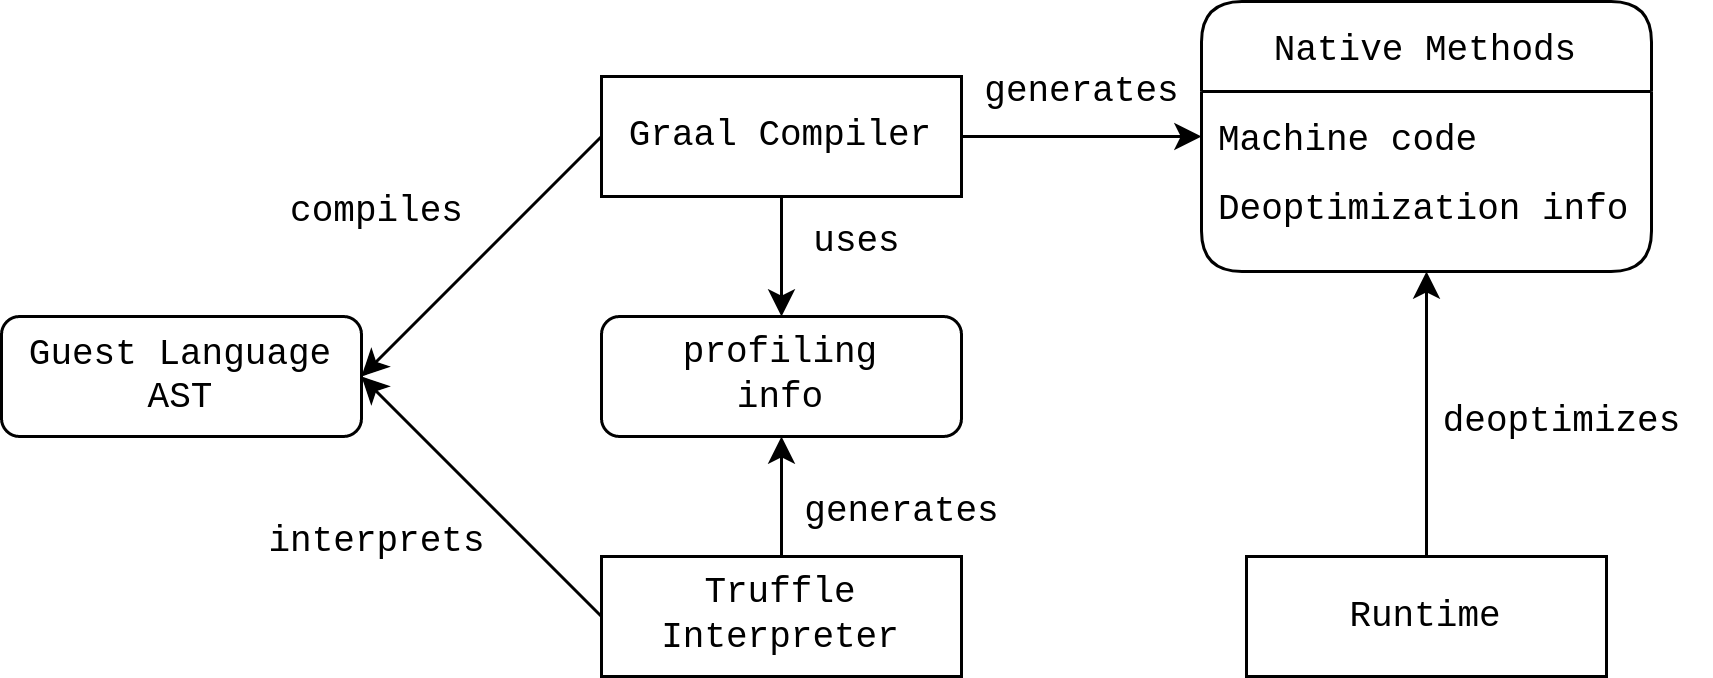
\includegraphics[width=0.5\textwidth]{figures/graalvm-pipeline.png}
	\caption{GraalVM overview\cite{graalvm:ir}.}
	\label{figure:graalvm-overview}
\end{figure}

Figure \ref{figure:graalvm-overview} provides an overview on the interactions between the multiple components of GraalVM.
This thesis makes substantial use of both components of GraalVM to create a runtime for Scala programs using TASTy.
The runtime is able to incorporate source level information for speculative optimizations.

\subsection{Graal}

GraalVM incorporates an existing implementation of a JVM\cite{java:hotspot} for the actual execution of programs.
Graal is \textit{only} the general-purpose just-in-time compilation infrastructure tt optimizes the programs to be executed.
Graal is general-purpose in that it conducts analysis and optimization on the same intermediate representation, \textit{Graal IR}, regardless of the source language.
Notably, most implementations of a source language utilizing GraalVM have an implementation in Truffle.
In addition to a Truffle interpreter for Java bytecode\cite{graalvm:espresso}, there is a direct translator for Java programs in GraalVM that parses Java bytecode into Graal IR.

Graal IR\cite{graalvm:ir} is an IR suitable for speculative optimizations, while still retaining information from the Truffle guest language AST.
Graal IR is based on the \textit{sea of nodes} concept\cite{click:sea-of-nodes} and satisfies the \textit{static single-assignment}\cite{ssa} property.
A sea of nodes is an abstraction based on a directed graph structure that relates the control-flow graph\cite{allen:ctrl-flow-analysis} of a program to its data-flow graph\cite{allen:data-flow-analysis}.
An intermediate representation is in single-static assignment form when each variable is defined before it is used.\cite{johnson:use-def-chains}.

GraalIR enables Graal to speculatively compile only the \textit{hot} branches\cite{graalvm:speculative-ir}, or branches that are most frequently taken in the control flow portion of the IR, and their transitive data dependencies.
When a compiled program violates any underlying assumptions, execution is \textit{deoptimized}\cite{self:deoptimization} and the program resumes execution in the interpreter.
Deoptimization occurs when the compiled program is no longer considered stable and valid.
Graal automatically inserts \textit{guard nodes} into the IR, which are conditional checks validating if speculative assumptions used to compile the program still hold.
Deoptimization is part of an execution loop between Graal and Truffle, which allows GraalVM to adapt aggressively and speculate to find the best optimization in a dynamic execution environment.

\subsection{Truffle}

\begin{figure}[!htb]
	\centering
	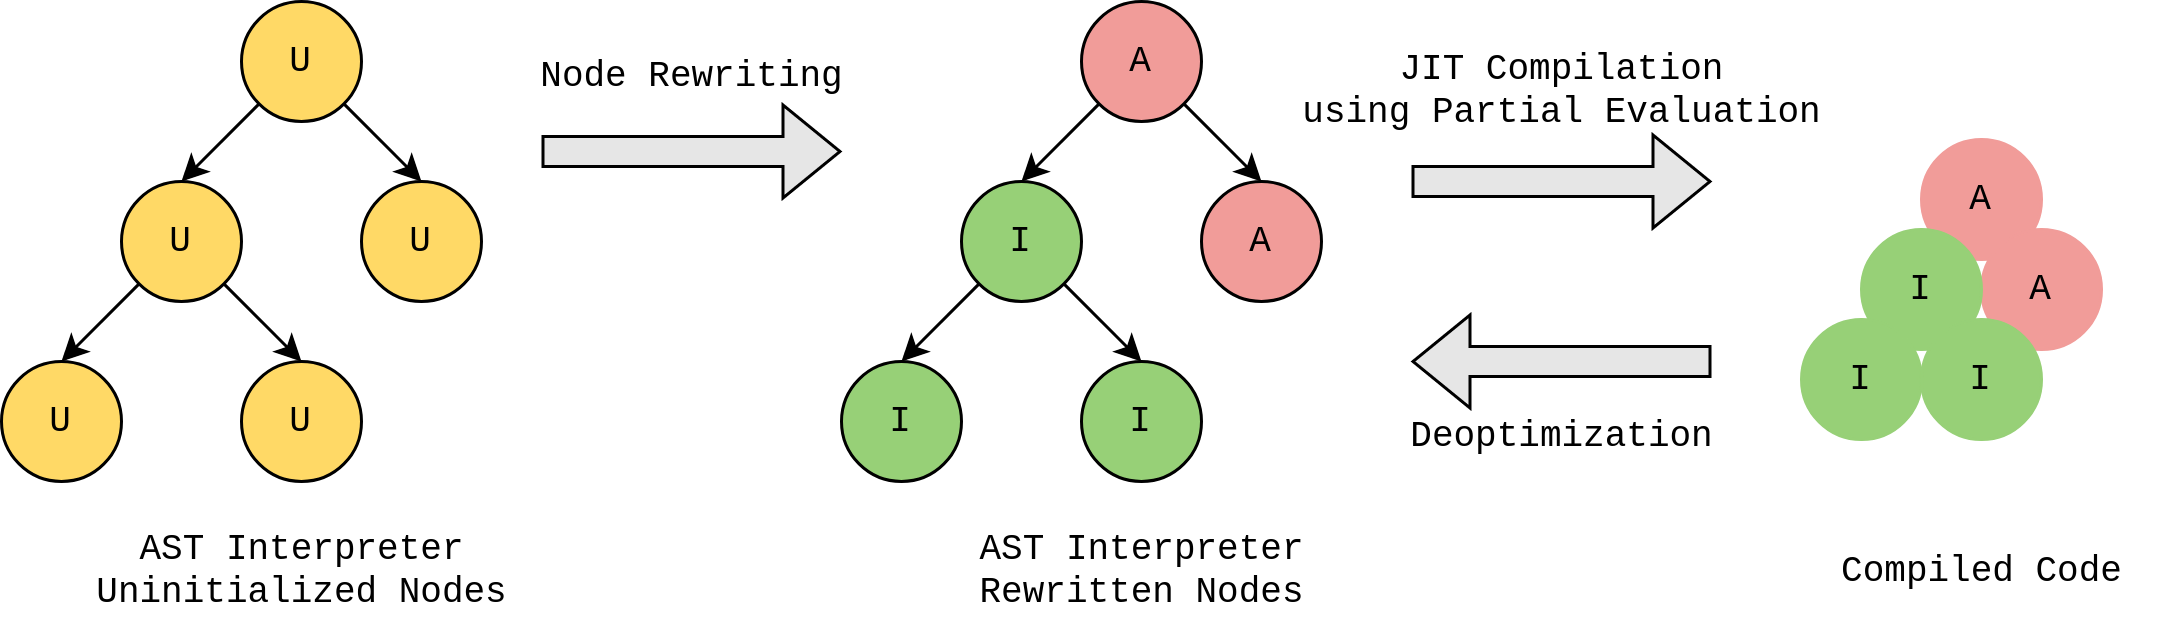
\includegraphics[width=0.75\textwidth]{figures/truffle-loop.png}
	\caption{Truffle's approach to self-optimization\cite{truffle:thesis}.}
	\label{diagram:graal-loop}
\end{figure}

Truffle is a framework for implementing an interpreter embedded into GraalVM.
Truffle differs significantly from other implementations of interpreters.
Interpreters can usually be divided into two subsets: tree interpreters and bytecode interpreters.
Tree interpreters transform the program source into an AST. 
AST interpretation has the added benefit of executing an intermediate representation close to the program source representation and is, therefore, more amenable to program optimization.
In contrast, bytecode interpreters, such as the JVM, execute a vastly simplified representation of programs.
While interpreters of bytecode programs tend to be faster than their tree counterparts, the absence of detailed source information, such as types, often makes program optimization difficult.
The problem of efficiently executing bytecode while retaining the ability to optimize them effectively using source program information is difficult for Scala on the JVM. 

Truffle is an atypical tree interpreter in that it combines the definition, execution, and optimization of an AST structure into a single abstraction.
While the structure of input programs in other interpreters is independent of the implementation of the interpreter, a Truffle interpreter is integrated into the structure of its input.
More concretely, this means an implementation of a Truffle interpreter is a collection of subclasses that extend \javainline{Node} class and implement a \javainline{execute()} method.
An interpreter is derived from implementing its input tree structure by defining execution semantics inside the AST to be executed.

During the execution of the AST, profiling information collected from the interpreter is used to drive \textit{node rewriting} and just-in-time compilation.
While Graal is language-agnostic, Truffle is able to exploit guest-language semantics for dynamic optimizations.
This process of replacing nodes in the AST with better, specialized guest-language counterparts in Truffle is called node rewriting.
Node rewriting makes Truffle abstract syntax trees self-optimizing and serves two purposes.
The first is to incorporate guestlanguage semantics into the executing program dynamically.
The second is to augment the AST for more efficient JIT compilation.
The nature of compiler optimizations requires that programs are incrementally simplified in order to be optimized.
While such types of optimizations are widely applicable to many languages using the JVM, node rewriting is a high-level language-specific optimization that occurs \textit{before} such simplifications.

The self-optimizing execution semantics of the AST are implemented with the Truffle \acrfull{dsl}.
The Truffle DSL is a mechanism to allow a \textit{guest language} to integrate semantics into a Truffle AST for self-optimization.
A guest language is a set of semantics, most commonly a programming language, encoded into a Truffle AST.
In this thesis, the guest language that our Truffle AST encodes and executes is TASTy (which represents Scala).

\begin{figure}[!htb]
\begin{minted}{scala}
abstract class EqualsNode extends BinaryOpNode {
	@Specialization
	def equalsInt(lhs: Int, rhs: Int): Boolean = lhs == rhs
	
	@Specialization
	def equals(lhs: Any, rhs: Any): Boolean = {
		if (lhs == null) 
		rhs == null 
		else 
		lhs.equals(rhs)
	}
}
\end{minted}
\caption{Pseudocode for a Truffle node implementation of an equality which supports node rewriting.}
\label{example:node-rewriting}
\end{figure}

Figure \ref{example:node-rewriting} demonstrates an example of the node that supports rewriting declared using the Truffle DSL.
The node declares semantics of the equality operation between integers and values of type \scalainline{Any}.
This equality node has semantics for every type because the \scalainline{Any} type is the supertype of all types in Scala.
A Truffle node that supports node rewriting begins in an uninitialized state.
When both the left and right-hand side operands are integers, the node is rewritten to \javainline{equalsInt} state.
When arguments of any other combination of types are detected, either in the uninitialized state or the \javainline{equalsInt} state, the node is rewritten to the \javainline{equals} state.


\begin{figure}[!htb]
\begin{minted}{java}
@GeneratedBy(EqualsNode.class)
public final class EqualsNodeGen extends EqualsNode {
	@Child private TermNode lhs_;
	@Child private TermNode rhs_;
	@CompilationFinal private int current_state;
	
	private EqualsNodeGen(TermNode lhs, TermNode rhs) {
		this.lhs_ = lhs;
		this.rhs_ = rhs;
	}
	
	public Object execute(VirtualFrame frame) {
		return (current_state & 2) != 0 && current_state != 0 ? 
			this.execute_int_int0(state, frame) : 
			this.execute_generic1(state, frame);
	}
	
	private Object execute_generic1(int state, VirtualFrame frame) {
		Object lhs = this.lhs_.execute(frame);
		Object rhs = this.rhs_.execute(frame);
		if ((state & 1) != 0 && lhs instanceof Integer) 
			if (rhs instanceof Integer) 
				return this.executeInt((Integer) lhs, (Integer) rhs);
		
		if ((state & 2) != 0) return this.executeObject(lhs, rhs);
		
		CompilerDirectives.transferToInterpreterAndInvalidate();
		return this.executeAndSpecialize(lhs, rhs);

	}	
}
\end{minted}
\caption{Generated code by the Truffle DSL for the \scalainline{AnyEqNode}.}
\label{impl:node-rewriting-gen}
\end{figure}

Figure \ref{impl:node-rewriting-gen} gives the auto-generated Java program that implements the semantics defined in \ref{example:node-rewriting}.
We will not discuss the semantics of every possible state in our generated node for brevity.
Instead, we will discuss the possible state transitions when a node starts in the uninitialized state.
State transitions are encoded as methods that execute the semantics for a given state, and update said state.
States are encoded as bit fields.
The uninitialized state is the $0$ value with no states encoded.
The \scalainline{equalsInt} state is encoded with $1$ and the \scalainline{equals} state is encoded with $2$.
\javainline{execute_generic1} is invoked when no states (specializations) are active in a \scalainline{EqualsNode}.
The first state transition checks whether the node is in one of two possible states (\scalainline{equalsInt} or \scalainline{equals}).
The corresponding specialization is invoked if the node is in either state and its arguments satisfy the preconditions.
This portion of the node may exist in either interpreted or compiled code.
However, if the node is not initialized, i.e., it is in neither possible state, the code is deoptimized (if compiled), and execution resumes from the interpreter.
While we do not showcase this, it is possible for a node to be in multiple states during execution.

The \javainline{executeAndSpecialize} method (figure \ref{impl:node-rewriting-specialize}) initializes the node to a specialized state.
If both arguments satisfy the \javainline{Int} type check invariant, the node is initialized to the \scalainline{equalsInt} state.
Otherwise, it is initialized to the \scalainline{equals} state.
Subsequent executions of the newly initialized node will invoke the appropriate specialization as long as their respective invariants are maintained.
Node rewriting narrows down a node's best implementation(s) for a particular profile of values.
If a Truffle AST cannot be rewritten further, it is considered \textit{stable}.
Stable nodes vastly simplify JIT compilation because of partial evaluation, a critical transformation applied to ASTs for JIT compilation that we will describe next.

\begin{figure}[!htb]
\begin{minted}{java}
private boolean executeAndSpecialize(Object lhs, Object rhs) {
	int prev_state = this.state_0_;
	if (lhs instanceof Integer) 
		if (rhs instanceof Integer) {
			this.current_state = prev_state |= 1;
			return this.equalsInt((Integer) lhs, (Integer) rhs);
		}

	this.current_state = prev_state |= 2;
	return this.equals(lhs, rhs);
}
\end{minted}
\caption{Implementation of \scalainline{executeAndSpecialize} of \scalainline{EqualsNodeGen}}
\label{impl:node-rewriting-specialize}
\end{figure}


When invocations of a root node exceed a predefined upper bound, Graal JIT compiles its children trees into native machine code using \textit{partial evaluation}.
Partial evaluation is a program optimization technique for specializing a program (code) for a given input (data)\cite{futamura:partial-eval}.
In the context of Truffle, this means specializing an AST node (code) based on the values, or types of values produced by their children nodes (data)\cite{truffle:partial-eval}.
The specialization of an AST node may also be based of the types of children nodes themselves.
We can say that the partial evaluation of an AST  will produce an AST that is \textit{specialized} for a particular set of values, or more commonly, in our case, a particular set of types.

For example, consider the partial evaluation of an \scalainline{EqualsNodeGen} node in the \scalainline{equalsInt} state.
The \javainline{current_state} field of the node is annotated with the \javainline{CompilationFinal} directive.
Truffle provides the \javainline{CompilationFinal} directive to indicate that a non-constant value in the guest-language implementation \textit{will} be a constant when being partially evaluated.
Because the state is a compilation constant, the condition on line $17$ of figure \ref{impl:node-rewriting-gen} evaluates to \javainline{true} when the state is $1$ (\scalainline{equalsInt}).
As a result, only the code for \javainline{execute_int_int0} (provided in \ref{impl:node-rewriting-state2}) will be compiled.
The generated implementation of \javainline{execute_int_int0} contains checks for the specialization invariant.
These checks act as points in the control flow of the compiled code to deoptimize, if these invariants are violated.
The resulting code supplied to the JIT compilation is the specialization of the \scalainline{EqualsNode} for the \scalainline{equalsInt} state.

\begin{figure}[!htb]
\begin{minted}{java}
private Object execute_int_int0(int state, VirtualFrame frame) {
	int lhs_int;
%	try {
		lhs_int = this.lhs_.executeInt(frame);
	} catch (UnexpectedResultException ex) {
		Object rhs = this.rhs_.execute(frame);
		return this.executeAndSpecialize(ex.getResult(), rhs);
	}
	
	int rhs_int;
	try {
		rhs_int = this.rhs_.executeInt(frame);
	} catch (UnexpectedResultException ex) {
		return this.executeAndSpecialize(lhs_int, ex.getResult());
	}
	
	assert (state & 1) != 0;
	return this.executeInt(lhs_int, rhs_int);
}
\end{minted}
\caption{Implementation of \scalainline{execute_int_int0} of \scalainline{EqualsNodeGen}}
\label{impl:node-rewriting-state2}
\end{figure}

The sequence of optimizations given in figure \ref{diagram:graal-loop}, node rewriting, partial evaluation, and deoptimization is the advantage that a TASTy Truffle interpreter has over the traditional JVM bytecode interpreter for Scala.
Truffle allows for the incorporation of source-level type information into the just-in-time compilation loop.
This thesis will focus on using these features to execute TASTy with type information to augment JIT compilation.

